\documentclass[a4paper, 11pt]{book}
% \usepackage{/home/nora/Documents/Enseignement/Prepa/bpep/fichiers_utiles/preambule}
\usepackage{cours-preambule}

\makeatletter
\renewcommand{\@chapapp}{Kh\^olles MPSI -- semaine}
\makeatother
\renewcommand\thechapter{26}

% \toggletrue{student}
% \toggletrue{corrige}

\begin{document}

\settype{enon}
\settype{solu}

\chapter{Sujet 1\siCorrige{\!\!-- corrig\'e}}

\resetQ
\section{Comparaison entre transformations}%
\enonce{%
	\noindent
	\begin{minipage}[c]{.10\linewidth}
		\begin{center}
			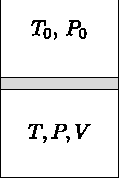
\includegraphics[width=\linewidth]{../figures/E6_intro}
		\end{center}
	\end{minipage}
	\hfill
	\noindent
	\begin{minipage}[c]{.85\linewidth}
		On considère un système composé d’une quantité de matière $n$ de gaz parfait
		diatomique enfermée dans une enceinte. Cette enceinte est fermée par un piston
		de surface $S$ et dont on négligera la masse, pouvant coulisser sans
		frottement. L’ensemble est situé dans l’atmosphère, dont on note $T_0$ et
		$P_0$ la température et la pression. On note I l’état initial. L’objectif est
		de comparer deux transformations du système : l’une brutale et l’autre lente.
		\smallbreak
		Commençons par la transformation brutale : on lâche brusquement une masse $M$
		sur le piston, qui se stabilise en un état intermédiaire $1$.
	\end{minipage}
}%

\QR{%
	Le meilleur modèle pour la transformation est-il isotherme ou adiabatique ?
	Peut-on en déduire un résultat sur la température $T_1$ ?
}{%
	Le système considéré est le gaz et l'enceinte autour. On s'intéresse à une
	transformation brusque. Le système n'a pas le temps d'échanger de l'énergie
	sous forme de transfert thermique avec l'extérieur : la transformation peut
	donc être considérée comme \textbf{adiabatique}. En revanche, comprimer un gaz
	rapidement le rend plus chaud (comme dans une pompe à vélo). La température du
	gaz va varier, la transformation \textbf{ne} sera donc \textbf{pas} isotherme.

	On ne peut rien dire sur $T_1$. On peut s'attendre à ce qu'elle soit
	supérieure à $T_0$ puisque l'on comprime rapidement le gaz.
}%
\QR{%
	Déterminer la pression $P_1$.
}{%
	À l'état $1$, le système est à l'équilibre mécanique. La pression qui s'exerce
	sur le piston est alors la somme de la pression atmosphérique plus celle de la
	masse posée sur la section $S$ du piston. On en déduit que :
	\[
		\boxed{P_1 = P_0+\frac{Mg}{S}}
	\]
}%

\QR{%
	Établir le bilan énergétique de la transformation en explicitant chacun des
	termes $W_{I\to 1}$, $Q_{I\to 1}$ et $\Delta_{I\to 1} U$, et appliquer le
	premier principe.
}{%
	Puisque cette transformation est considérée comme adiabatique :
	\[
		\boxed{Q_{I\to 1} = 0}
	\]
	La transformation qu’il subit est monobare : tout au long de cette
	transformation, la pression extérieure est celle exercée par le piston sur le
	gaz qui est constante (la masse $M$ est déposée en
	bloc). Ainsi,
	\[
		W_{I\to 1} = -P\ind{ext}\Delta{V}
		\Lra
		\boxed{W_{I\to 1} = -\left(P_0+\frac{Mg}{S}\right)(V_1-V_I)}
	\]

	Comme le gaz est parfait, il suit la première loi de \textsc{Joule}, donc
	\[
		\Delta{U}_{I\to 1} = C_V\Delta{T}
		\Lra
		\boxed{\Delta_{I\to 1} U = \frac{5}{2}nR(T_1 - T_I)}
	\]
	D'après le premier principe appliqué au système pendant la transformation $I
		\to 1$~:
	\[
		\Delta{U}_{I\to 1} = W_{I\to 1}
		\Lra
		\boxed{\frac{5}{2}nR (T_1 - T_I) = - \left( P_0 + \frac{Mg}{S} \right)(V_1
			- V_0)}
	\]
}%

\QR{%
	Exprimer alors $T_1$ en fonction des pressions $P_1,P_0$ et la température
	$T_0$, et $V_1$ en fonction des pressions et du volume $V_I = V_0$.
}{%
	La pression $P_1$ est déjà connue. Pour déterminer la température $T_1$, on
	peut remplacer les volumes par $V_i = nRT_i/P_i$ dans l'expression du premier
	principe. Sachant que l'état initial est un état d'équilibre, on a $T_I = T_0$
	et, \textbf{sans la masse}, $P_I = P_0$. Ainsi, on trouve
	\begin{gather*}
		\frac{5}{2}nR (T_1 - T_I) = -nRP_1 \left( \frac{T_1}{P_1} - \frac{T_I}{P_I} \right)
		\qqdc
		\boxed{T_1 = \frac{2}{7}\left( \frac{5}{2}+\frac{P_1}{P_I} \right)T_I}
		\\\Lra
		\underbracket[1pt]{nRT_1}_{P_1V_1} =
		\frac{2}{7}\left( \frac{5}{2}+\frac{P_1}{P_I} \right)\underbracket[1pt]{nRT_0}_{P_0V_0}
		\quad \Lra \quad
		\boxed{V_1 = \frac{2}{7} \left( \frac{5P_0}{2P_1} + 1 \right)V_0}
	\end{gather*}
}%

\enonce{%
	On observe qu’en fait l’état 1 n’est pas un réel état d’équilibre : le piston
	continue de bouger, mais beaucoup plus lentement, jusqu’à atteindre l’état 2
	qui est l’état final.
}%

\QR{%
	Quel phénomène, négligé précédemment, est responsable de cette nouvelle
	transformation du système ? Comment peut-on qualifier cette transformation~?
}{%
	On a négligé les transfert d'énergie thermique entre le gaz et l'extérieur.
	\smallbreak
	Cette transformation peut alors être qualifiée de \textbf{monobare} et
	\textbf{monotherme} (la température et la pression de l'extérieur ne varient
	pas). On peut aussi considérer que cette transformation est \textbf{isobare}
	car, comme la \textbf{transformation est lente}, le système sera à chaque
	instant à l'équilibre mécanique avec l'extérieur.
}%

\QR{%
	Déterminer les caractéristiques $T_2$, $P_2$, $V_2$ de l’état 2.
}{%
	Dans l’état final, l’équilibre est complètement atteint~: il y a équilibre
	thermique et mécanique.  D'après la question précédente :
	\[
		\boxed{T_2 = T_0}
		\qqet
		\boxed{P_2=P_0+\frac{Mg}{S}}
	\]
	Le volume occupé par le gaz est imposé par la loi du gaz parfait :
	\[
		\boxed{V_2 = \frac{nRT_2}{P_2} = \frac{nRT_0}{P_0+\frac{Mg}{S}}}
	\]
}%

\QR{%
	Déterminer le travail reçu par le système, puis sa variation d’énergie interne
	au cours de la transformation $1\to 2$. En déduire le travail total et le
	transfert thermique total reçus au cours de la transformation brusque.
}{%
	Le travail des forces de pression a cours de $1 \to 2$ se calcule comme
	précédemment~:
	\begin{align*}
		W_{1\to 2}          & =
		- \left( P_0 + \frac{Mg}{S} \right) (V_2-V_1)
		\\
		\beforetext{et on a}
		\Delta{U}_{1 \to 2} & = \frac{5}{2}nR (T_2-T_1)
		\intertext{Le transfert thermique reçu s'obtient alors par}
		Q_{1\to 2}          & =
		\Delta{U}_{1\to 2} - W_{1\to 2}
		\\ &=
		\underbracket[1pt]{\frac{5}{2}nR
			(\underbracket[1pt]{T_2}_{=T_0}-T_1)}_{=-W_{I\to 1}} +
		\left( P_0 + \frac{Mg}{S} \right) (V_2-V_1)
		\\\Lra
		\Aboxed{Q_{1\to 2}  & = \left( P_0 + \frac{Mg}{S} \right) (V_2-V_0)}
	\end{align*}
	Finalement, le travail total et le transfert thermique total reçus au cours de
	la transformation brusque valent~:
	\[
		W\ind{tot} = - \left( P_0 + \frac{Mg}{S} \right) (V_2-V_0)
		\qet
		Q\ind{tot} = \left( P_0 + \frac{Mg}{S} \right) (V_2-V_0)
	\]
	Ainsi, on a évidemment $W\ind{tot} + Q\ind{tot} = 0$~: en effet, dans l'état
	$I$ et l'état final $2$, le gaz est en équilibre thermique avec l'extérieur à
	$T_0$~; or $\Delta{U} = C_V\Delta{T}$ donc $\Delta{U} = W\ind{tot} +
		Q\ind{tot} = 0$~!
}%
\enonce{%
	Comparons maintenant à une transformation lente~: la même masse $M$ est lâchée
	très progressivement sur le piston, par exemple en ajoutant du sable «~grain à
	grain~».
}%
\QR{%
	Comment qualifie-t-on une telle transformation~? Que peut-on en déduire sur la
	température du système au cours de la transformation~?
}{%
	On la dit \textbf{quasi-statique}. On peut suppose qu'elle laisse largement le
	temps aux échanges thermiques d'avoir lieu, si bien que l'équilibre thermique
	est atteint à tout instant. Par conséquent, on peut considérer la
	transformation \textbf{isotherme}~: $T = T_0$.
}%
\QR{%
	Déterminer la pression dans l'état final et en déduire le volume. Commenter.
}{%
	Dans l'état final $F$, la masse placée sur le piston est exactement la même que
	dans le cas précédent~: on en déduit
	\[
		\boxed{P_F = P_2 = P_0 + \frac{Mg}{S}}
	\]
	et comme par ailleurs $T_F = T_0 = T_2$, avec la loi du gaz parfait on a
	également $V_F = V_2$. Ainsi, \textbf{les états finaux sont les mêmes}. Cela
	n'a rien d'étonnant~: les équilibres thermique et mécanique sont établis dans
	les 2 états, et les contraintes extérieures (masse $M$, pression $P_0$ et
	température $T_0$) sont les mêmes.
}%
\QR{%
	Établir le bilan énergétique de la transformation en explicitant chaque terme.
}{%
	La transformation étant quasi-statique, on a $P = P\ind{ext}$, soit
	\begin{gather*}
		W = -\int_{V_i}^{V_f} P\ind{ext}\dd{V} = -\int_{V_i}^{V_f} P \dd{V}
		\\\Lra
		W = -nRT_0 \int_{V_i}^{V_f} \frac{\dd{V}}{V} \Lra
		\boxed{W = -nRT_0 \ln \frac{V_f}{V_i}}
	\end{gather*}
	Par ailleurs, la transformation étant isotherme on a $\Delta{U} = C_V\Delta{T}
		= 0$, et avec le premier principe
	\[
		\Delta{U} = W+Q \Lra Q = -W
		\qso
		\boxed{Q = nRT_0 \ln \frac{V_f}{V_i}}
	\]
	On voit ainsi que les deux transformations ont les mêmes états initial et
	final, donc la même variation d'énergie interne, alors que les échanges
	d'énergie ne sont pas les mêmes.
}%
\QR{%
	Représenter alors ces deux transformations dans un diagramme de \textsc{Watt}
	$(P,V)$, en considérant la transformation $I\to 1$ mécaniquement réversible,
	et commenter.
}{%
	\vspace{-30pt}
	\begin{center}
		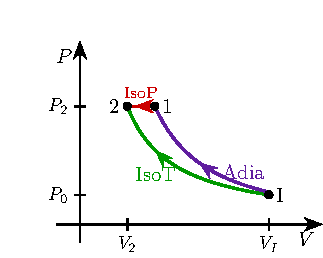
\includegraphics[width=.4\linewidth]{../figures/E6_adia_vs_isoT}
	\end{center}
}%

\chapter{Sujet 2\siCorrige{\!\!-- corrigé}}
\resetQ
\subimport{/home/nora/Documents/Enseignement/Prepa/bpep/exercices/TD/corps_humain/}{sujet.tex}

\chapter{Sujet 3\siCorrige{\!\!-- corrigé}}
\resetQ
\subimport{/home/nora/Documents/Enseignement/Prepa/bpep/exercices/TD/calorimetrie_2/}{sujet.tex}

% \chapter{Sujet 3\siCorrige{\!\!-- corrig\'e}}
% \resetQ
% \subimport{/home/nora/Documents/Enseignement/Prepa/bpep/exercices/TD/cycle_Carnot/}{sujet.tex}

% \chapter{Sujet 4\siCorrige{\!\!-- corrig\'e}}
% \resetQ
% \subimport{/home/nora/Documents/Enseignement/Prepa/bpep/exercices/DS/adiabatique_isotherme/}{sujet.tex}

\chapter{Sujet 4\siCorrige{\!\!-- corrig\'e}}
\resetQ
\subimport{/home/nora/Documents/Enseignement/Prepa/bpep/exercices/TD/thermometre_gaz/}{sujet.tex}

\chapter{Sujet 5\siCorrige{\!\!-- corrig\'e}}
\resetQ
\subimport{/home/nora/Documents/Enseignement/Prepa/bpep/exercices/TD/interpretation_microscopique_loi_des_gaz_parfaits/}{sujet.tex}

\end{document}
